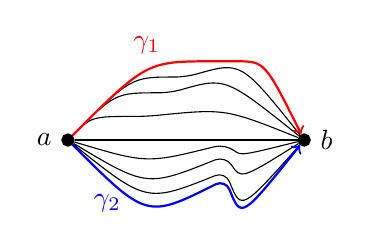
\begin{tikzpicture}
    \tikzstyle{point}=[circle,thick,draw=black,fill=black,inner sep=0pt,minimum width=4pt,minimum height=4pt]
    \node (a)[point,label=180:$a$] at (0,0) {};
    \node (b)[point,label=0:$b$]   at (3, 0) {};
    \draw [rounded corners] (a) .. controls (0.8,0.8) .. (1.5,0.8) .. controls (2.2,1) .. (b);
    \draw [rounded corners] (a) .. controls (0.6,0.6) .. (1.3,0.6) .. controls (2.0,0.8) .. (b);
    \draw [rounded corners] (a) .. controls (0.3,0.3) .. (1.0,0.3) .. controls (2.0,0.4) .. (b);
    \draw [rounded corners] (a) -- (b);
    \draw [rounded corners] (a) .. controls (1,-0.8) .. (2,-0.4) .. controls (2.2,-0.9) .. (b);
    \draw [rounded corners] (a) .. controls (1,-0.6) .. (2,-0.2) .. controls (2.2,-0.5) .. (b);
    \draw [rounded corners] (a) .. controls (1,-0.3) .. (2,-0.05) .. controls (2.2,-0.2) .. (b);
    \draw [rounded corners,->, thick, red] (a) .. controls (1,1) .. (2,1) .. controls (2.5,1) .. (b);
    \draw [rounded corners,->, thick, blue] (a) .. controls (1,-1) .. (2,-0.5) .. controls (2.2,-1) .. (b);
    \node at (1,1.2) [red] {$\gamma_1$};
    \node at (0.5,-0.8) [blue] {$\gamma_2$};
\end{tikzpicture}
